\documentclass[12pt]{article}
\usepackage{amsfonts, amssymb, amsmath, amsthm}
\usepackage[margin=1in]{geometry}
\usepackage{tikz}

\title{Explainer: Problem 5 (Rudin 7.3) --- Products Don't Preserve Uniform Convergence}
\author{}
\date{}

\begin{document}
\maketitle

\section*{The challenge}
Build two sequences $\{f_n\}$, $\{g_n\}$ where:
\begin{itemize}
  \item $f_n \to f$ uniformly on some set $E$,
  \item $g_n \to g$ uniformly on $E$,
  \item BUT $f_n g_n \to fg$ only \emph{pointwise}, not uniformly.
\end{itemize}

\textbf{Context (from Problem 7.2):} If both sequences are uniformly bounded, uniform convergence \emph{is} preserved by products. So your counterexample must involve at least one \textbf{unbounded} sequence.

\section*{Why unboundedness breaks things}
Uniform convergence means $\sup_x |f_n(x) - f(x)| \to 0$. For the product:
$$
f_n g_n - fg = (f_n - f) g_n + f(g_n - g).
$$
The first term is small in sup-norm \emph{only if} $g_n$ is bounded. If $g_n(x)$ grows large somewhere, a tiny error $(f_n - f)$ can be amplified enormously.

\section*{Classic recipe}
Take $E = \mathbb{R}$ (or any unbounded set).
\begin{itemize}
  \item $f_n(x) = \frac{1}{n}$ (constants, $\to 0$ uniformly).
  \item $g_n(x) = x$ (no $n$-dependence, $\to x$ ``uniformly'' trivially).
\end{itemize}
Then $f_n g_n = x/n \to 0$ pointwise, but
$$
\sup_{x \in \mathbb{R}} \left| \frac{x}{n} - 0 \right| = +\infty
$$
for every $n$. So the convergence is not uniform.

\begin{center}
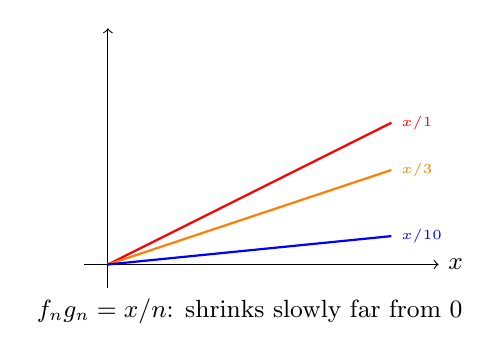
\begin{tikzpicture}[scale=0.6]
  \draw[->] (-0.5, 0) -- (7, 0) node[right] {\small $x$};
  \draw[->] (0, -0.5) -- (0, 5);
  \draw[thick, red] (0,0) -- (6, 6/2) node[right] {\tiny $x/1$};
  \draw[thick, orange] (0,0) -- (6, 6/3) node[right] {\tiny $x/3$};
  \draw[thick, blue] (0,0) -- (6, 6/10) node[right] {\tiny $x/10$};
  \node at (3, -1) {\small $f_n g_n = x/n$: shrinks slowly far from $0$};
\end{tikzpicture}
\end{center}

\section*{Alternative recipe}
You could also use $f_n(x) = x + 1/n$ (with $f(x) = x$) and $g_n(x) = 1/n$ (with $g = 0$): then $f_n g_n = x/n + 1/n^2$, same issue. The point is to keep one factor \emph{unbounded} while the other shrinks.

\section*{Takeaway}
Uniform convergence is a statement about the \emph{worst-case} pointwise error, measured in sup-norm. Multiplication by an unbounded function can blow up a uniformly-small error into a uniformly-large error.

\end{document}
